\documentclass[10pt,a4paper]{article}
\usepackage{amsmath}
\usepackage{amsfonts}
\usepackage{amssymb}
\usepackage{natbib}
\usepackage{graphicx}
\usepackage[left=2cm,right=2cm,top=2cm,bottom=2cm]{geometry}
\usepackage{arydshln}

\title{Validating Plate Boundary Observatory borehole strainmeter data with GNSS derived strain} 
\author{Trever T. Hines and Eric A. Hetland}
\begin{document}

\maketitle


\section{Introduction}\label{sec:Introduction}
The Plate Boundary Observatory (PBO) maintains 82 borehole strain meters (BSMs), most of which are installed along the Western United States. BSMs are able to detect geophysical processes such as coseismic and postseismic deformation \citep[e.g.,][]{Langbein2006,Langbein2015}, slow slip events \citep[e.g.,][]{Dragert2011}, and seismic wave propagation \citep{Barbour2017}. BSMs are intended for measuring deformation over timescales of minutes to months. At longer timescales, BSM data is contaminated by factors such as borehole relaxation \citep{Gladwin1987}. Slow slip events and postseismic deformation occur on timescales that near the upper limit of what BSMs can be expected to resolve. Another complication with BSM data is that the strain measured at the borehole may deviate from the regional strain due to local topographic or geologic features \citep{Berger1976}. Due to these sources of noise, it can be difficult to use BSM data quantitatively in, for example,  geophysical inverse problems. In this study, we assess the ability of BSMs to measure strain resulting from slow slip events (SSEs) on the Cascadia subduction zone. This is done by comparing BSM data to strain derived from GNSS data. 

There are about forty BSMs in the Pacific Northwest and only five of them, B003, B004, B005, B007, and B018, record noticeable deformation from SSEs. Of these stations B005 and B007 are collocated. We show that only station B004 produces strain that is in reasonable agreement with GNSS derived strain rates.  Station B018 records shear strains with opposite polarity as the GNSS derived strains. This discrepancy can be explained by an $25^\circ$ error in the recorded orientation of the instrument. 

GNSS derived strains are computed with Gaussian process regression using the method described in \citep{Hines2017}.   

\section{BSM Data}
The are about forty PBO BSMs in the Pacific Northwest, and only five of them, B003, B004, B005, B007, and B018, record noticeable deformation from SSEs. We limit our attention to these five station in this study.  The remaining stations either contain too much noise on the timescale of SSEs or are too far away from the SSEs to observe any strain. Each of the PBO BSMs are Gladwin four-component tensor strainmeters, which are about 2 m long, 8.7 cm in diameter, and are installed at about 100 to 200 m depth. Each BSM contains four extensometers, or gauges. Only three gauges are necessary to completely determine the horizontal strain tensor, and the fourth gauge is included for redundancy. Gauges 1, 2, and 3 are oriented $60^\circ$, $120^\circ$, and $150^\circ$ counterclockwise from gauge 0.   

We use the level 2 gauge data provided by UNAVCO at www.unavco.org, which has undergone several post-processing steps. In the level 2 gauge data a borehole curing trend is estimated and removed by fitting two exponential terms and a linear trend to the data. The level 2 data is corrected for tidal strains by estimating and removing sinusoids with known tidal frequencies. There is also a correction for barometric pressure because the normal stress imposed on the surface by barometric pressure results in horizontal strains recorded by the BSM. The barometric pressure correction is the observed barometric pressure at each site multiplied by a best fitting scaling factor. Lastly, offsets have been removed in the level 2 data product.    

We denote the extension measured at gauge $i$ as $e_i$, and the strain tensor components as $\varepsilon_{xx}$, $\varepsilon_{yy}$, and $\varepsilon_{xy}$, where $x$ and $y$ indicate the east and north direction, respectively. The extensions measured at BSMs are traditionally converted into areal strain, $\varepsilon_a = \varepsilon_{xx} + \varepsilon_{yy}$, differential strain $\varepsilon_d = \varepsilon_{xx} - \varepsilon_{yy}$, and engineering shear strain, $\varepsilon_s = 2\varepsilon_{xy}$. In this study, we will compare $\varepsilon_a$, $\varepsilon_d$, and $\varepsilon_s$ recorded at the BSMs to those predicted by GNSS data. Using $\theta_0$ to denote the orientation of gauge 0, in degrees north of east, these strain components can be expressed in terms of the gauge measurements through the equation 
\begin{equation}\label{eq:GaugeToStrain}
\left[\begin{array}{c}
\varepsilon_a \\
\varepsilon_d \\
\varepsilon_s \\
\end{array}\right]
=
2\mathbf{K}^{-1}\left[\begin{array}{ccc}
1 & \cos(2\theta_0) & \sin(2\theta_0) \\
1 & \cos(2(\theta_0 + 60)) & \sin(2(\theta_0 + 60)) \\
1 & \cos(2(\theta_0 + 120)) & \sin(2(\theta_0 + 120)) \\
1 & \cos(2(\theta_0 + 150)) & \sin(2(\theta_0 + 150)) \\
\end{array}\right]^+
\left[\begin{array}{c}
e_0 \\
e_1 \\
e_2 \\
e_3 \\
\end{array}\right],
\end{equation} 
where ``$+$" indicates the Moore-Penrose pseudoinverse and $\mathbf{K}$ is a coupling matrix describing how the instrument strains relate to the crustal strains \citep{Hart1996}. In this paper $\varepsilon_a$, $\varepsilon_d$, and $\varepsilon_s$ are ideally intended to represent crustal strains. We assume that BSMs are installed in homogeneous, isotropic rock, allowing us to write the coupling matrix as
\begin{equation}\label{eq:CouplingMatrix}
\mathbf{K} = 
\left[\begin{array}{ccc}
c & 0 & 0 \\
0 & d & 0 \\
0 & 0 & d \\
\end{array}\right],
\end{equation}  
where $c$, and $d$ are response factors that depend on the elastic properties of the instrument, the grout, and surrounding rock \citep{Gladwin1985}. Based on the analysis of \citet{Gladwin1985}, we use $c=1.5$ and $d=3.0$. UNAVCO, the organization responsible for maintaining the PBO BSMs and disseminating their data, use these same response factors for their final data products. 

Local topographic or geologic features can cause $\mathbf{K}$ to have non-zero off diagonal elements. If possible, the components of $\mathbf{K}$ should be determined in-situ by calibrating the BSM data with a well known strain source, such as diurnal and semi-diurnal tides \citep{Hart1996,Roeloffs2010,Hodgkinson2013}. \citet{Hart1996} calibrated a BSM at Pinyon Flat, using the tidal strains recorded at a collocated laser strain meter. This calibration method is, of course, not possible for most PBO BSMs. \citet{Roeloffs2010} and \citet{Hodgkinson2013} calibrated PBO BSMs using theoretical predictions of tidal strains \citep[e.g.,][]{Agnew1997}. This approach is still not adequate for BSMs near large local bodies of water, which can make it difficult to form an accurate theoretical estimate of tidal strains. As determined by \citet{Roeloffs2010}, the five BSM stations considered in this paper are too close to the Straight of Juan de Fuca to be accurately calibrated with tidal strains. Since in-situ calibration is not possible, we acknowledge that our choice for $\mathbf{K}$ is likely to be a significant source of error in BSM data. Another potential source of error is the assumed orientation for $\theta_0$. This orientation is determined by a compass on the instrument, and it is possible that magnetic minerals in the surrounding rock can give the compass an erroneous reading. 

\section{GNSS derived strain}
We compare the BSM strain components to transient strains estimated from GNSS data. In this paper, transient strain is considered to be any deviation from the steady rate of strain accumulation from plate tectonics.  We use daily GNSS displacement solutions for 94 continuous GNSS stations in the Pacific Northwest (Figure 1). The data is available from www.unavco.org. We convert the GNSS data to transient strains using Gaussian process regression (GPR) as described in \citet{Hines2017a}. With GPR, we select a prior spatio-temporal covariance model for the geophysical signal that we want to recover. Following \citet{Hines2017a}, we assume that our prior for displacements is a Gaussian process with zero mean, and covariance function described by 
\begin{equation}\label{cov}
C_u((t,x),(t',x')) = \phi^2 T(t,t')X(x,x'),
\end{equation}        
where $T$ is the Wendland covariance function
\begin{equation}\label{eq:Wendland}
T(t,t') = \left(1 - \frac{|t - t'|}{\tau}\right)^5_+ \left(\frac{8|t - t'|^2}{\tau^2} + \frac{5|t - t'|}{\tau} + 1\right), 
\end{equation}
and $X$ is the squared exponential covariance function
\begin{equation}\label{eq:SE}
X(\vec{x},\vec{x}') = \exp\left(\frac{-||\vec{x} - \vec{x}'||_2^2}{2 \ell^2}\right).
\end{equation}
The hyperparameters $\phi$, $\tau$, and $\ell$ control the amplitude, characteristic time-scale, and characteristic length-scale of the prior. \citet{Hines2017a} found that the optimal hyperparameters for describing displacements from SSEs are roughly $\phi =$ 0.5 mm, $\tau =$ 0.1 yr, and $\ell =$ 100 km. These parameters were chosen objectively using maximum likelihood methods; however based on our experience, this prior may not be sufficiently flexible to described all the observed data. Consequently, we explore using lower values for $\tau$ and $\ell$ and a higher value for $\phi$. For each tested set of hyperparameters, we condition the prior with the observed GNSS data and visually compare the posterior displacements to the observations. We settle on the values $\phi = 1.0$ mm, $\tau =$ 0.05 yr, and $\ell =$ 80 km. With this final set of hyperparameters, we condition the prior with the GNSS data and then spatially differentiate the posterior displacements to obtain transient strain.

\section{Results}
We compare the BSM data to GNSS derived strains for seven SSEs. The earliest SSE occurred in spring 2009 and the latest SSE occurred in 2017. The two datasets are in best agreement for the summer 2010 SSE (Figure \ref{fig:SSE1}). We only show the differential and engineering shear strains because there is no clear signal in the areal strain for either the GNSS derived strains or the BSM data. \citet{Roeloffs2010} also expressed doubt in the areal strains measured at stations B003, B004, B007, and B018 because the areal strains derived from different combinations of gauges at these stations are not self consistent. \citet{Roeloffs2010} also noted an self inconsistency in the differential strains at B003. 

Station B004 record differential and engineering shear strains that are most consistent with the GNSS derived strains. However, the first sign of SSE strains recorded at B004 tend to lag about five days behind the GNSS derived strains. The strain rates recorded at B004 also tend to be greater than the GNSS derived strains. One possible explanation for this discrepancy is that the GNSS station spacing is too wide to resolve a relatively sharp pulse of strain from the SSE as it traverses along the subduction zone. The engineering shear strains recorded at B003 are also in good agreement with the GNSS derived strains, although there are similar discrepancies between the timing and strain rates.

Stations B005 and B007, which are located within a few hundred meters of eachother, both show a clear SSE signal in their engineering shear strains.  However, the temporal pattern of strain recorded at these stations are not consistent with the GNSS derived strains.  For the summer 2010 SSE, the GNSS derived strains predict a single positive pulse of engineering shear strain at these locations, but both B005 and B007 record an initially positive pulse that then becomes negative. We cannot explain this discrepancy with mis-oriented instruments because both B005 and B007 would need to have nearly identical orientation errors. If the negative pulse of engineering shear strain were a regional ($\gtrsim$50 km scale) feature, then it would have been recognized in the GNSS data. We then suspect that the discrepancy can be explained with topographic of geologic features that may distort the local strain field. While, we are not saying that the engineering shear strains at B005 and B007 are erroneous, it is clear that they are inconsistent with the regional scale strains. The differential strains at station B005 and B007 do not show any clear SSE signal, even though the GNSS data predicts that there should be. This too could perhaps be due to distortion of the strain field from local features.

The differential and engineering shear strains recorded station B018 are notably absent of noise. However, the engineering shear strains at B018 are not consistent with the GNSS derived strains. For example, BSM data shows a strain increase from the summer 2010 SSE, and the GNSS derived strains predict a strain decrease with about equal magnitude. In the next section we attempt to remediate this inconsistency by assuming that the recorded orientation is erroneous. 

tdhe two datasets describe opposite changes in the engineering shear strain changes from the summer 2010 SSE.    

    

The magnitude and    

 If it was real, this negative pulse of shear strain should have been seen in the GNSS data, based on the magnitude and duration of the negative shear strain, this  should have been clearly observable from the GNSS        

  

  be biased towards underestimating the    It is possible that the spacing of GNSS stations in this region is too wide to resolve the relatively sharp pulse of strain    


\section{Reorienting B018}     

\begin{figure}
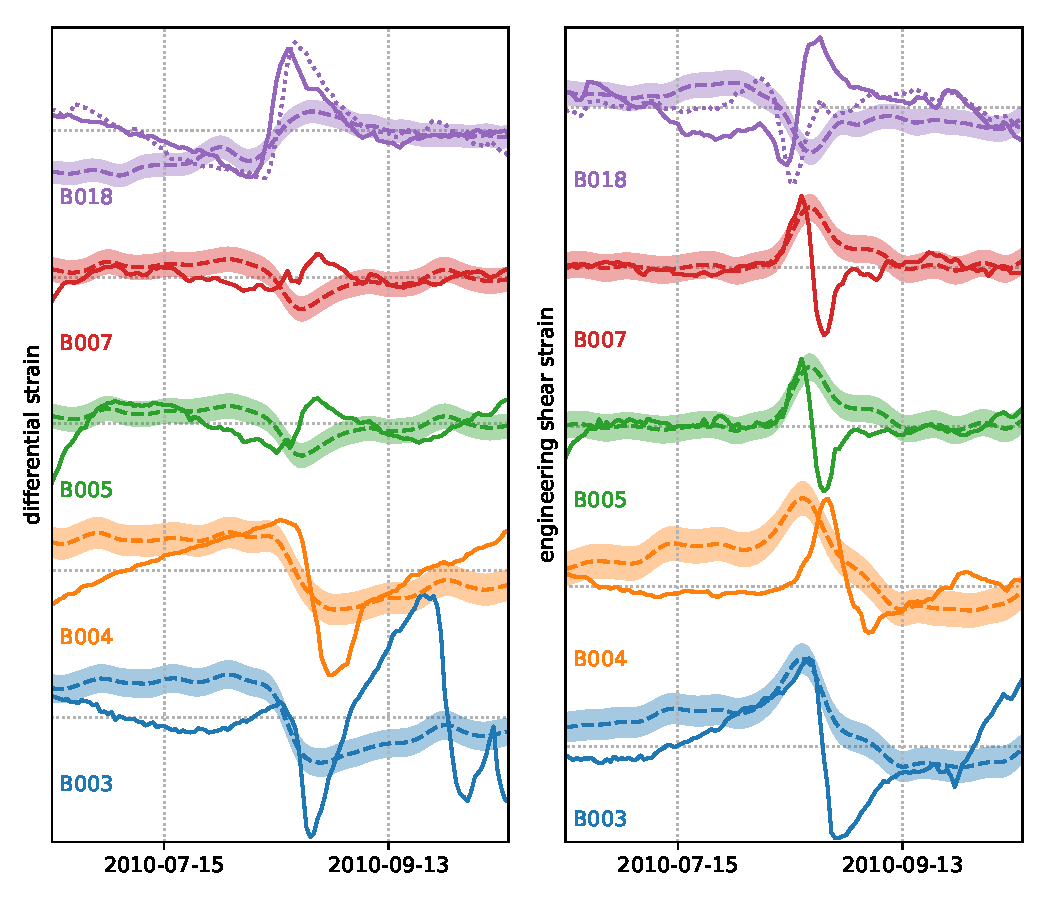
\includegraphics[scale=1.0]{figures/SSE1.pdf}
\caption{foo}   
\label{fig:SSE1}
\end{figure}

\bibliographystyle{apalike}
\bibliography{mybib}  
 
\end{document}